\section{Results}

\subsection{Comparison with null models}

\begin{figure}[H]
    \centering
    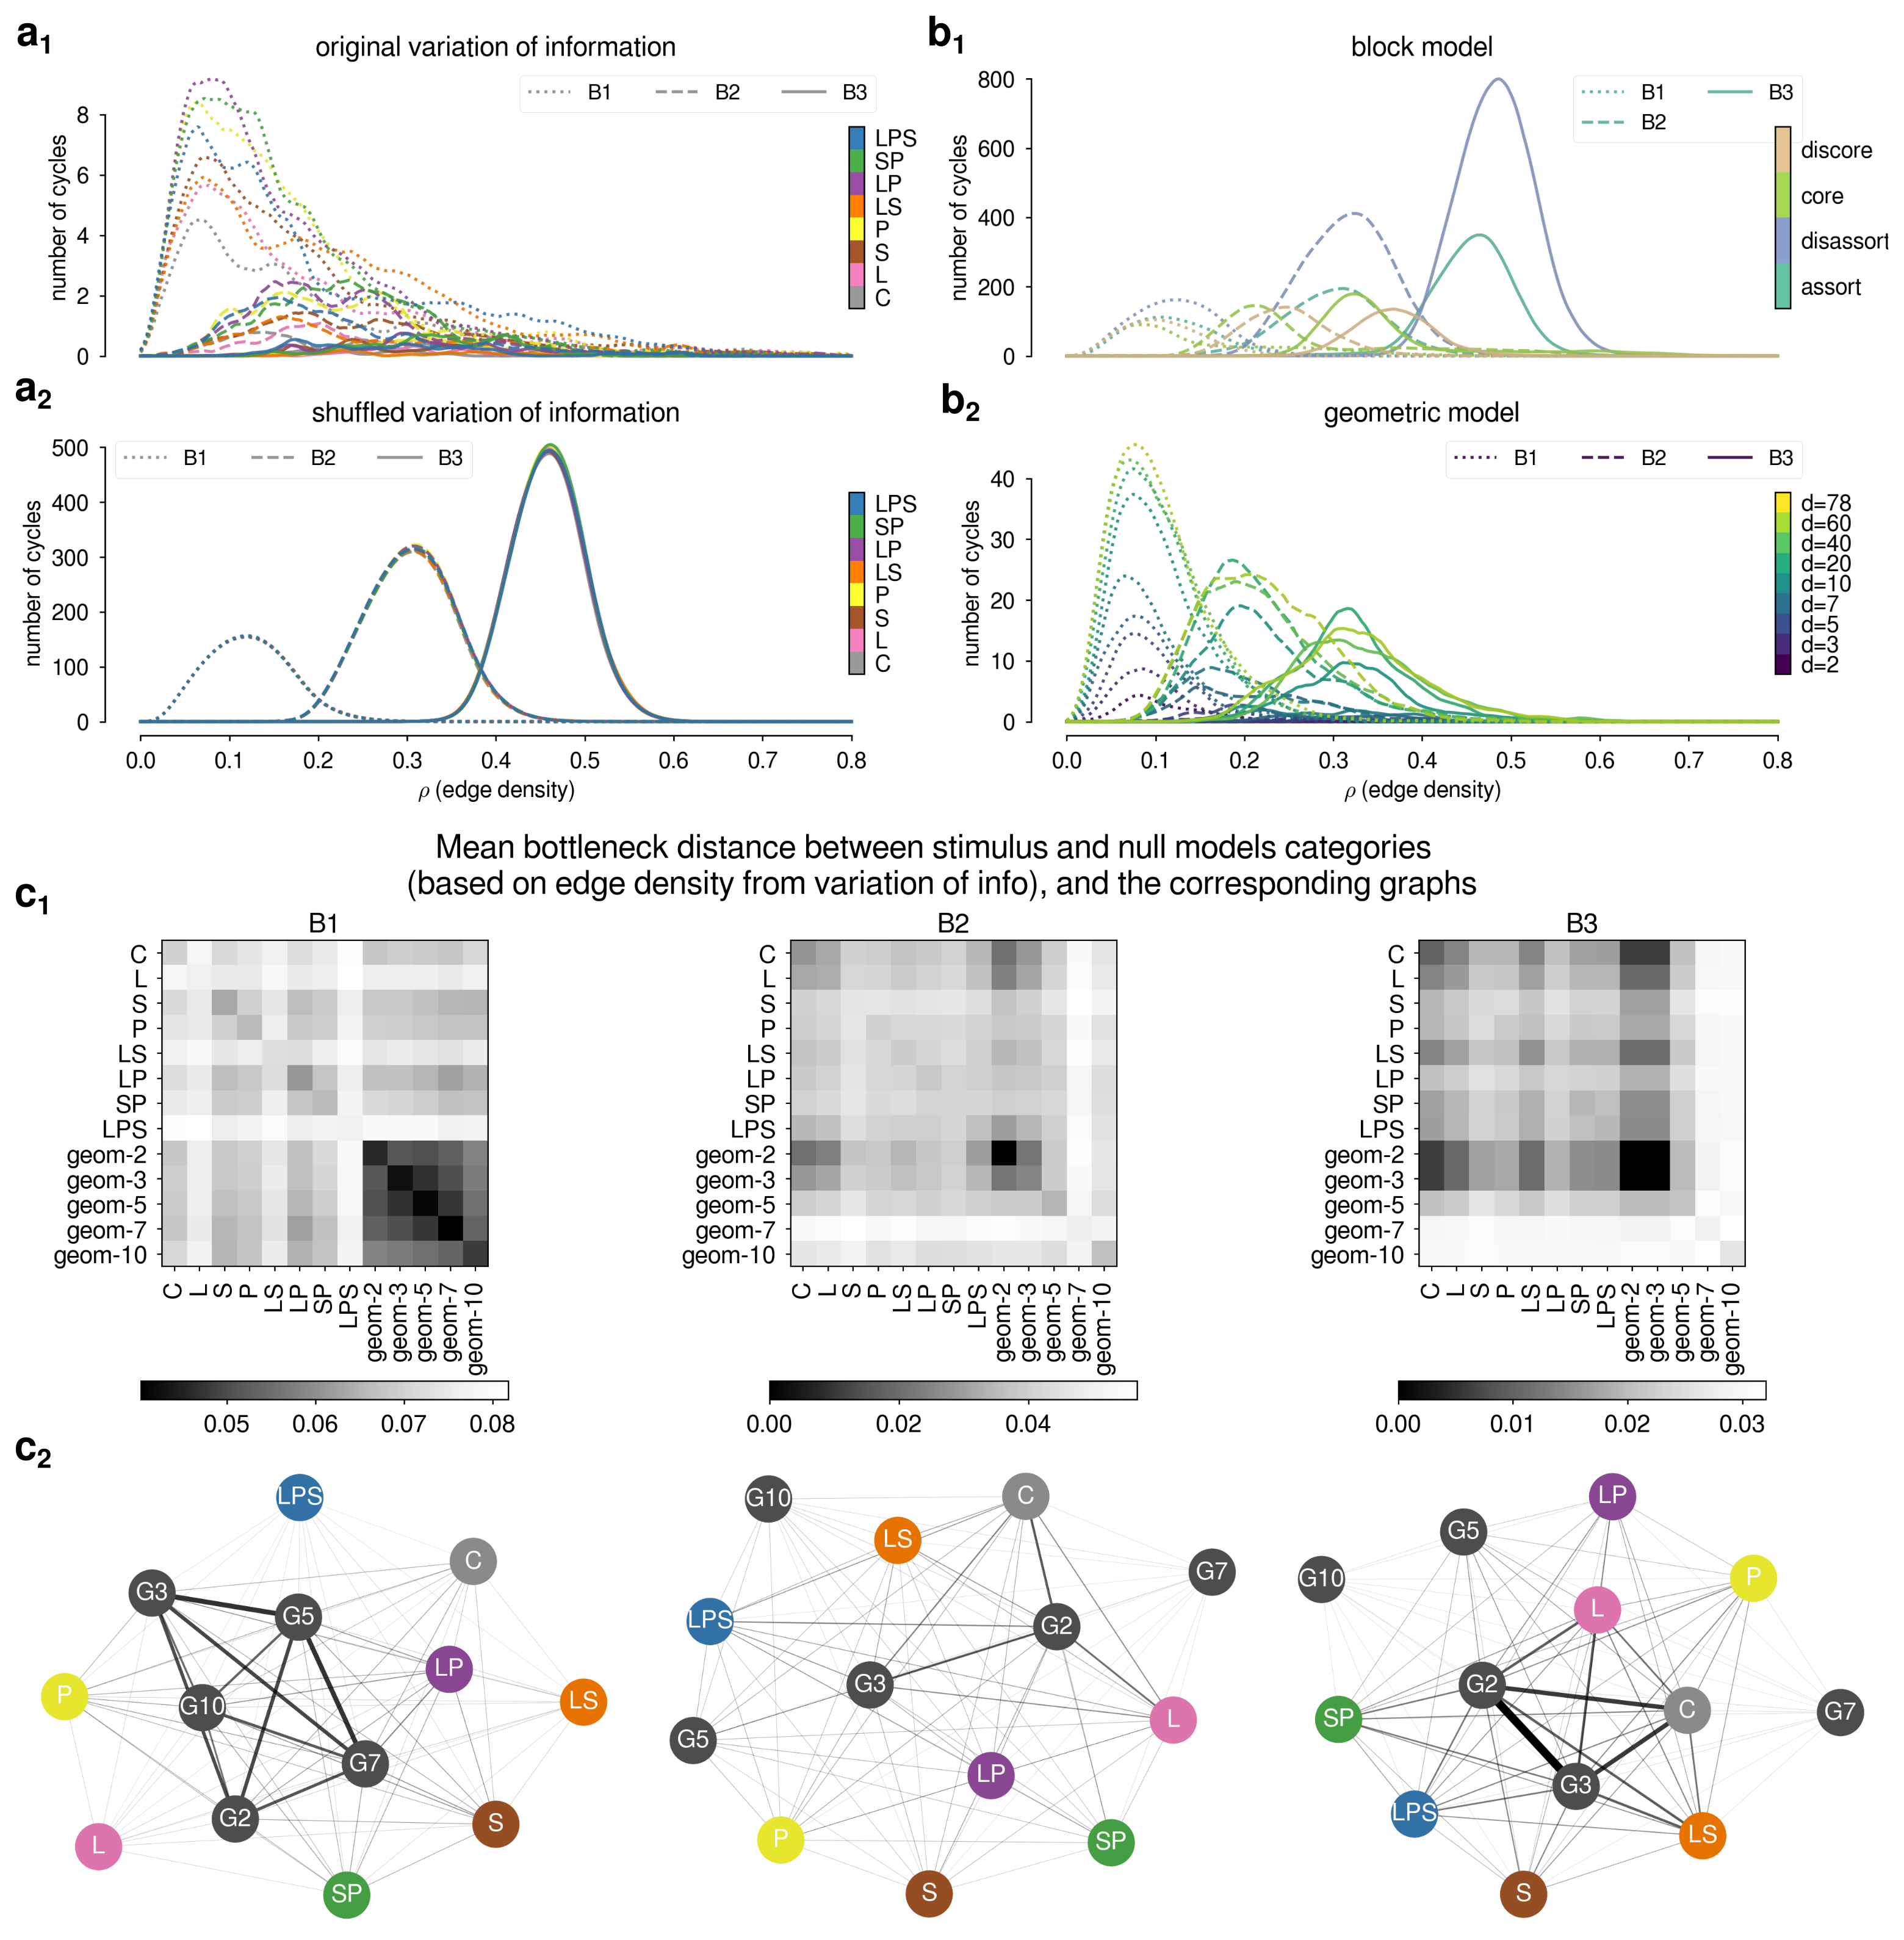
\includegraphics[width=0.8\textwidth,center]{../figures/report/Fig3.png}
    \caption{\label{fig:3}
    \textit{Comparison of Betti curves and bottleneck distances between Purkinje population topology and different null models}.
    (\textbf{a}) Mean Betti curves as a function of edge density of the original data (a$_1$) and the shuffled (a$_2$) variation of information matrix data. Colors are different stimulus categories.
    (\textbf{b}) Mean Betti curves of the block null models (b$_1$, colors represent different block configurations) and the geometric models (b$_2$, colors represent different dimensions).
    (\textbf{c}) Mean bottleneck distance matrix (c$_1$) between different stimulus categories and a select few geometric null models; and the graphs (c$_2$) constructed from converting these distance matrix to similarity matrix (i.e. thickness of edge means smaller bottleneck distance).
    }
\end{figure}

With the Betti curves as a function of edge density, I can compare the topology of the original data with the different null models, as well as with the shuffled versions of the data distance matrices representing an IID null.

First off, the original Purkinje cell population topology is different from the IID null, via comparison of the Betti curves (\autoref{fig:3}a$_{1,2}$) and the integrated Betti numbers (\autoref{fig:4}a$_{1}$), suggesting that there exists some meaningful topology in the data and not completely random. This is similar to the observations made in hippocampal data \cite{Giusti2015-uo}.

\begin{figure}[H]
    \centering
    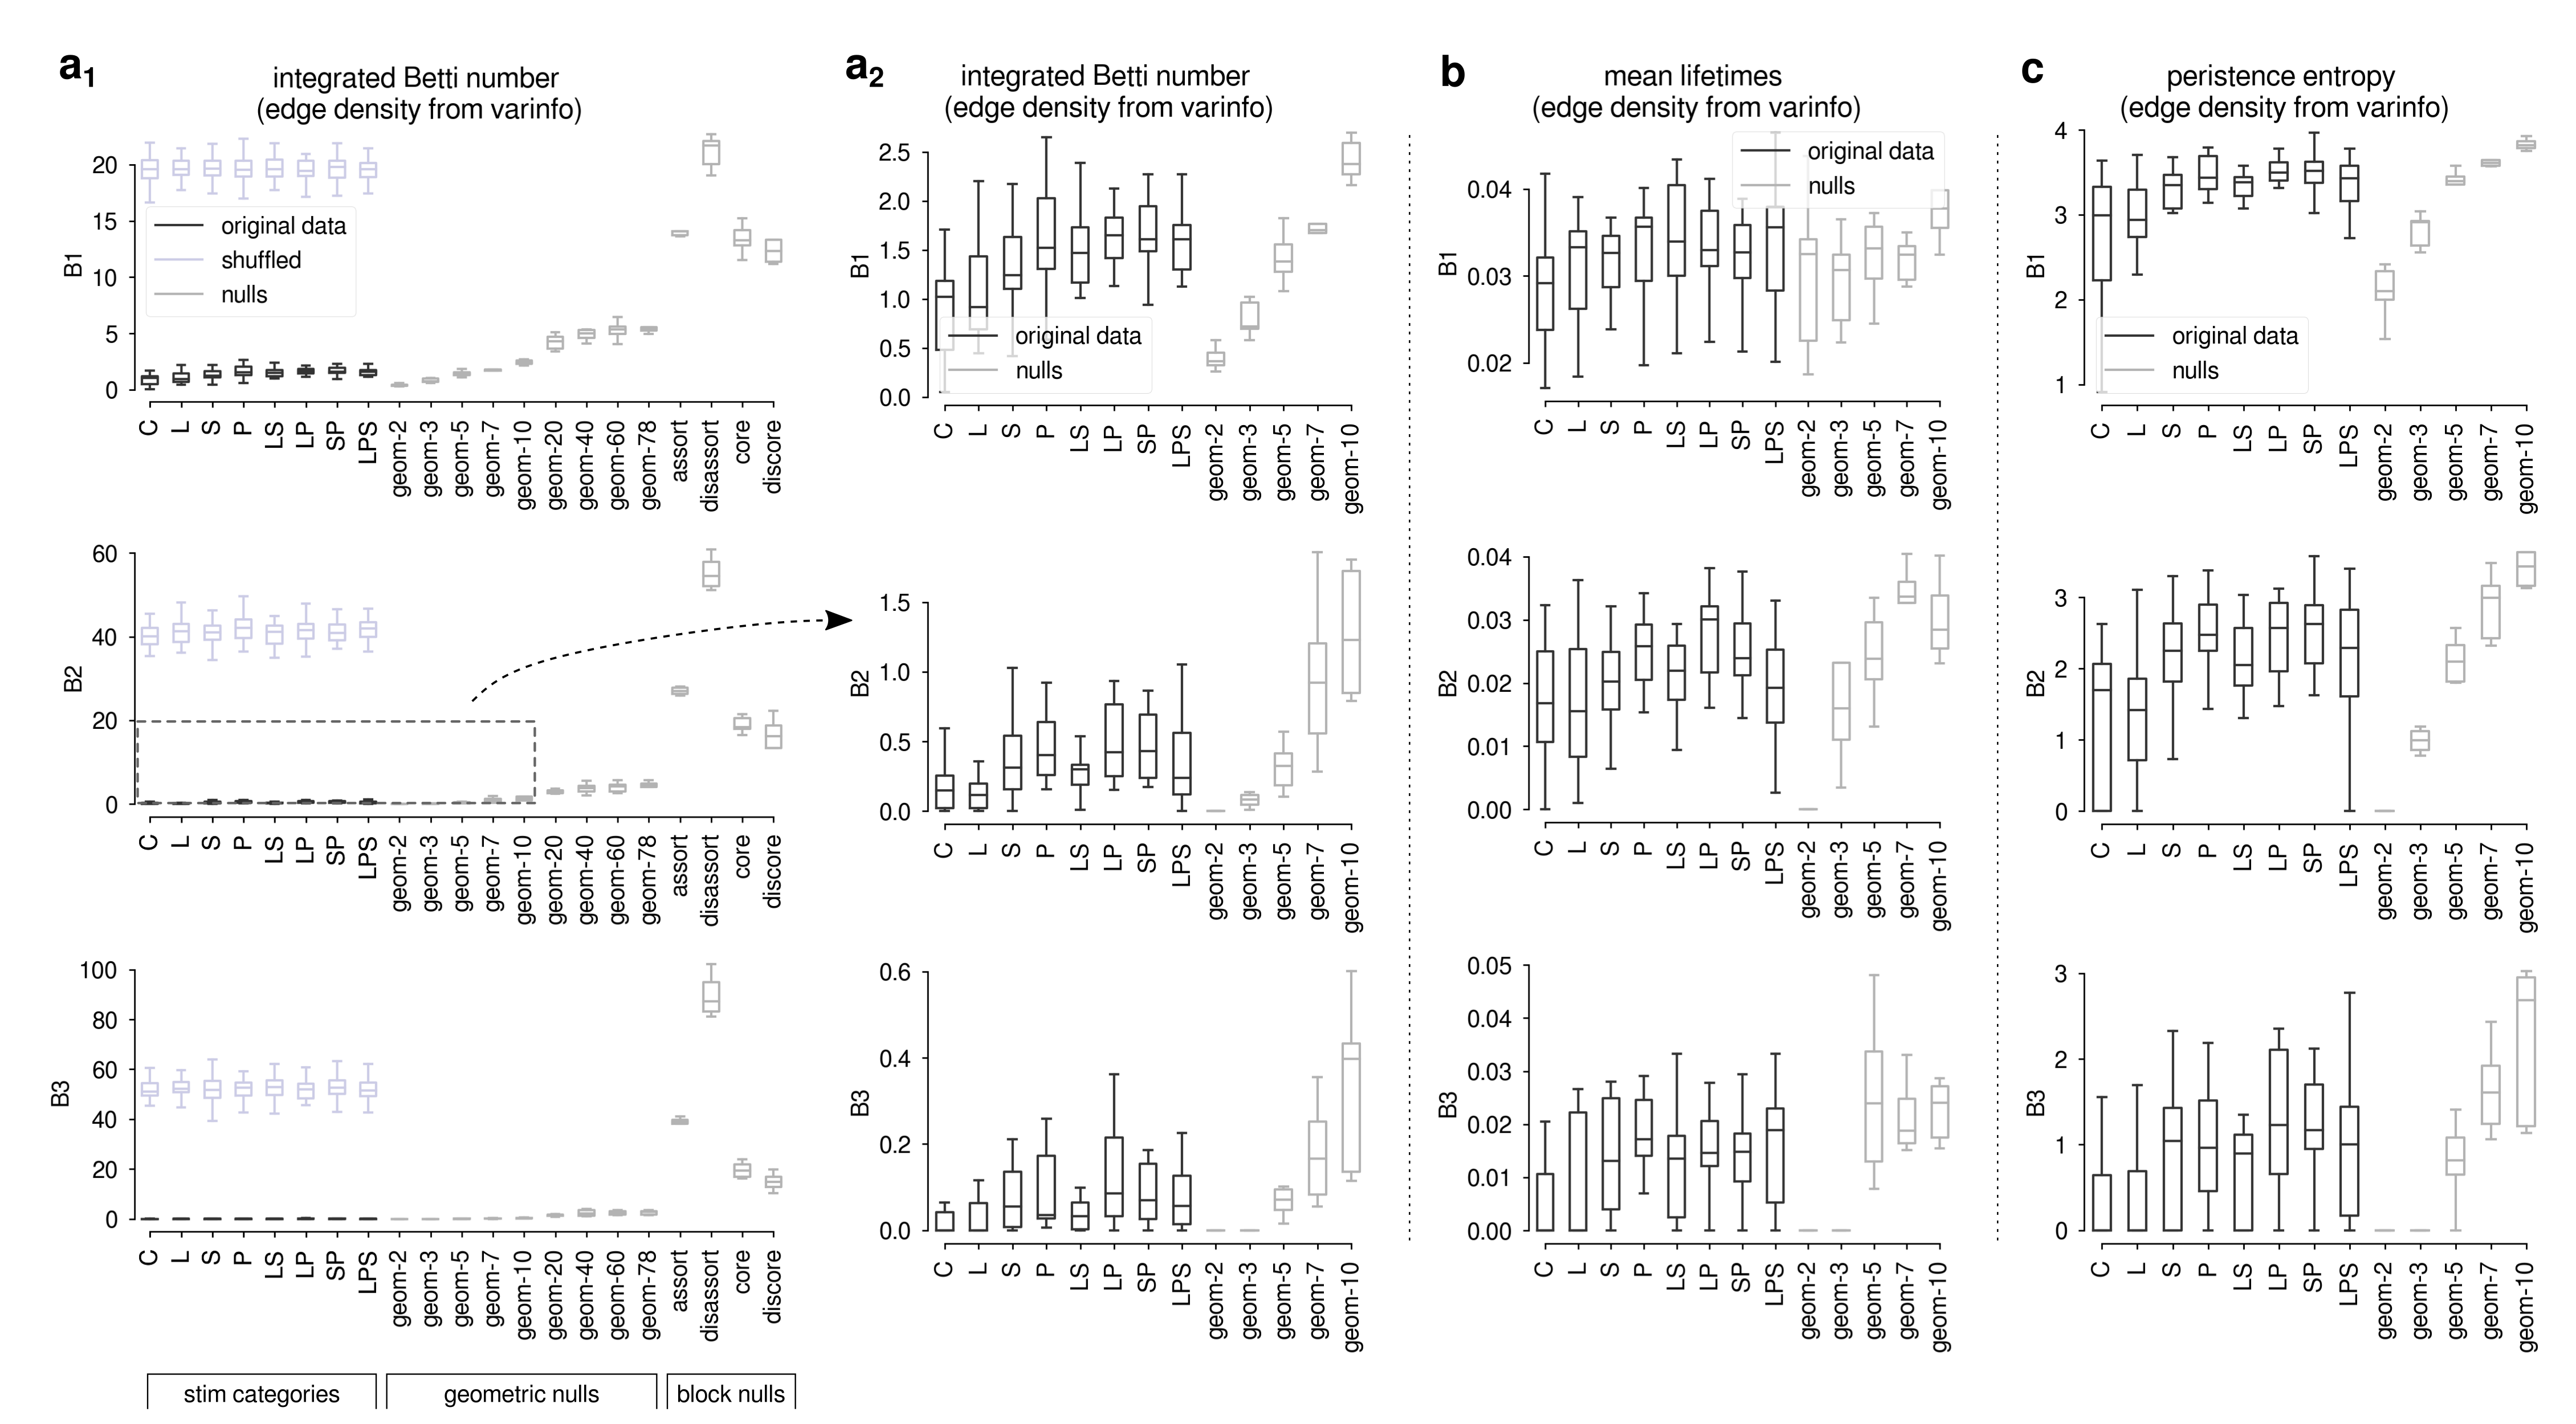
\includegraphics[width=\textwidth,center]{../figures/report/Fig4.png}
    \caption{\label{fig:4}
    \textit{Title}.
    Descriptions
    }
\end{figure}

Secondly, the topology of the population does not seem to resemble any of the block models as the number of cycles of these models are quite large and do not decrease with homology dimensions compared to original data (compare \autoref{fig:3}a$_1$ and b$_1$). Hence, the integrated Betti numbers for these block models across dimensions would tend to be much larger than those of the original data. It is possible that if such block topology exists, it is much smaller. A way to test this in the future would be to consider more blocks or smaller number of elements per block.

Thirdly, when comparing with geometric models like done in \cite{Giusti2015-uo}, the analysis reveals some similarity between the Purkinje information network topology and geometric topology of low dimensions. This is supported with the overall decreasing number of cycles with increasing homology dimensions (compare \autoref{fig:3}a$_1$ and b$_2$). However, I observe that the similarity, if it exists, would only exist for geometric models of dimensions less than 10. This is supported by inspecting the integrated Betti number, mean lifetimes and persistent entropy in \autoref{fig:4}. This is in contrast to the topology of the hippocampal place cell topology observed in \cite{Giusti2015-uo}, where similarity is observed in higher geometric model dimensions as well.

Additionally, upon closer inspection between the different stimulus categories and low-dimensional geometric models using the bottleneck distances (\autoref{fig:3}c), trials associated with C or L are more similar to lower dimensions geometric models in $B_2$ (also somewhat recapitulated in \autoref{fig:4}a$_2$ middle panel), while all of them are closer to \texttt{geom} $\le 5$ in $B_3$.

In summary, the analysis shows that there possible exists geometric topology of low dimensions (possible 2-10) in the Purkinje population either at spontaneous condition (no stimuli) or with stimulus. It is unclear whether block topology exists in the data at this point. Future endeavors require inspection of smaller blocks, as well other possible null models like a few mentioned in \cite{Blevins2021-tf}.

\subsection{Comparison across different stimulus categories}

I want to compare across different stimulus categories to see whether topology features could be used to decode out the different sensory conditions the animal was in. Inspecting using edge density does not reveal much ``structure'' in the bottleneck distance matrices (\autoref{fig:3}c). Additionally, it is possible that comparison using the actual distance is better: for example, a control (C) trial might reveal the same topology but with lower connectivity strength than a stimulus trial, and comparing the Betti curves as a function of the distance parameter without conversion to edge density might be more insightful for decoding. Hence, I repeated the analysis and extended it to also $B_0$.

Inspecting the mean Betti curves (\autoref{fig:5}a) reveals that control (C) and light (L) trials generally evoke fewer cycles than other stimulus conditions (but C is still $<$ than L), in all dimensions as the curves for the former two reach maximum and decrease earlier than the latter. Sound (S) and puff (P) trials seem to create more cycles generally, either with higher Betti curve peaks or wider curves. The combinations of stimulus modalities have interesting effects on the Betti curves in $B_1,B_2$ (certain trends also follow in $B_3$ but much noisier). For example, the presence of L brings down or shifts left the curve when combined with either S or P. Additionally, the presence of P is usually accompanied with high Betti curve peaks. When all three modalities are present, the results are much more mixed.

\begin{figure}[H]
    \centering
    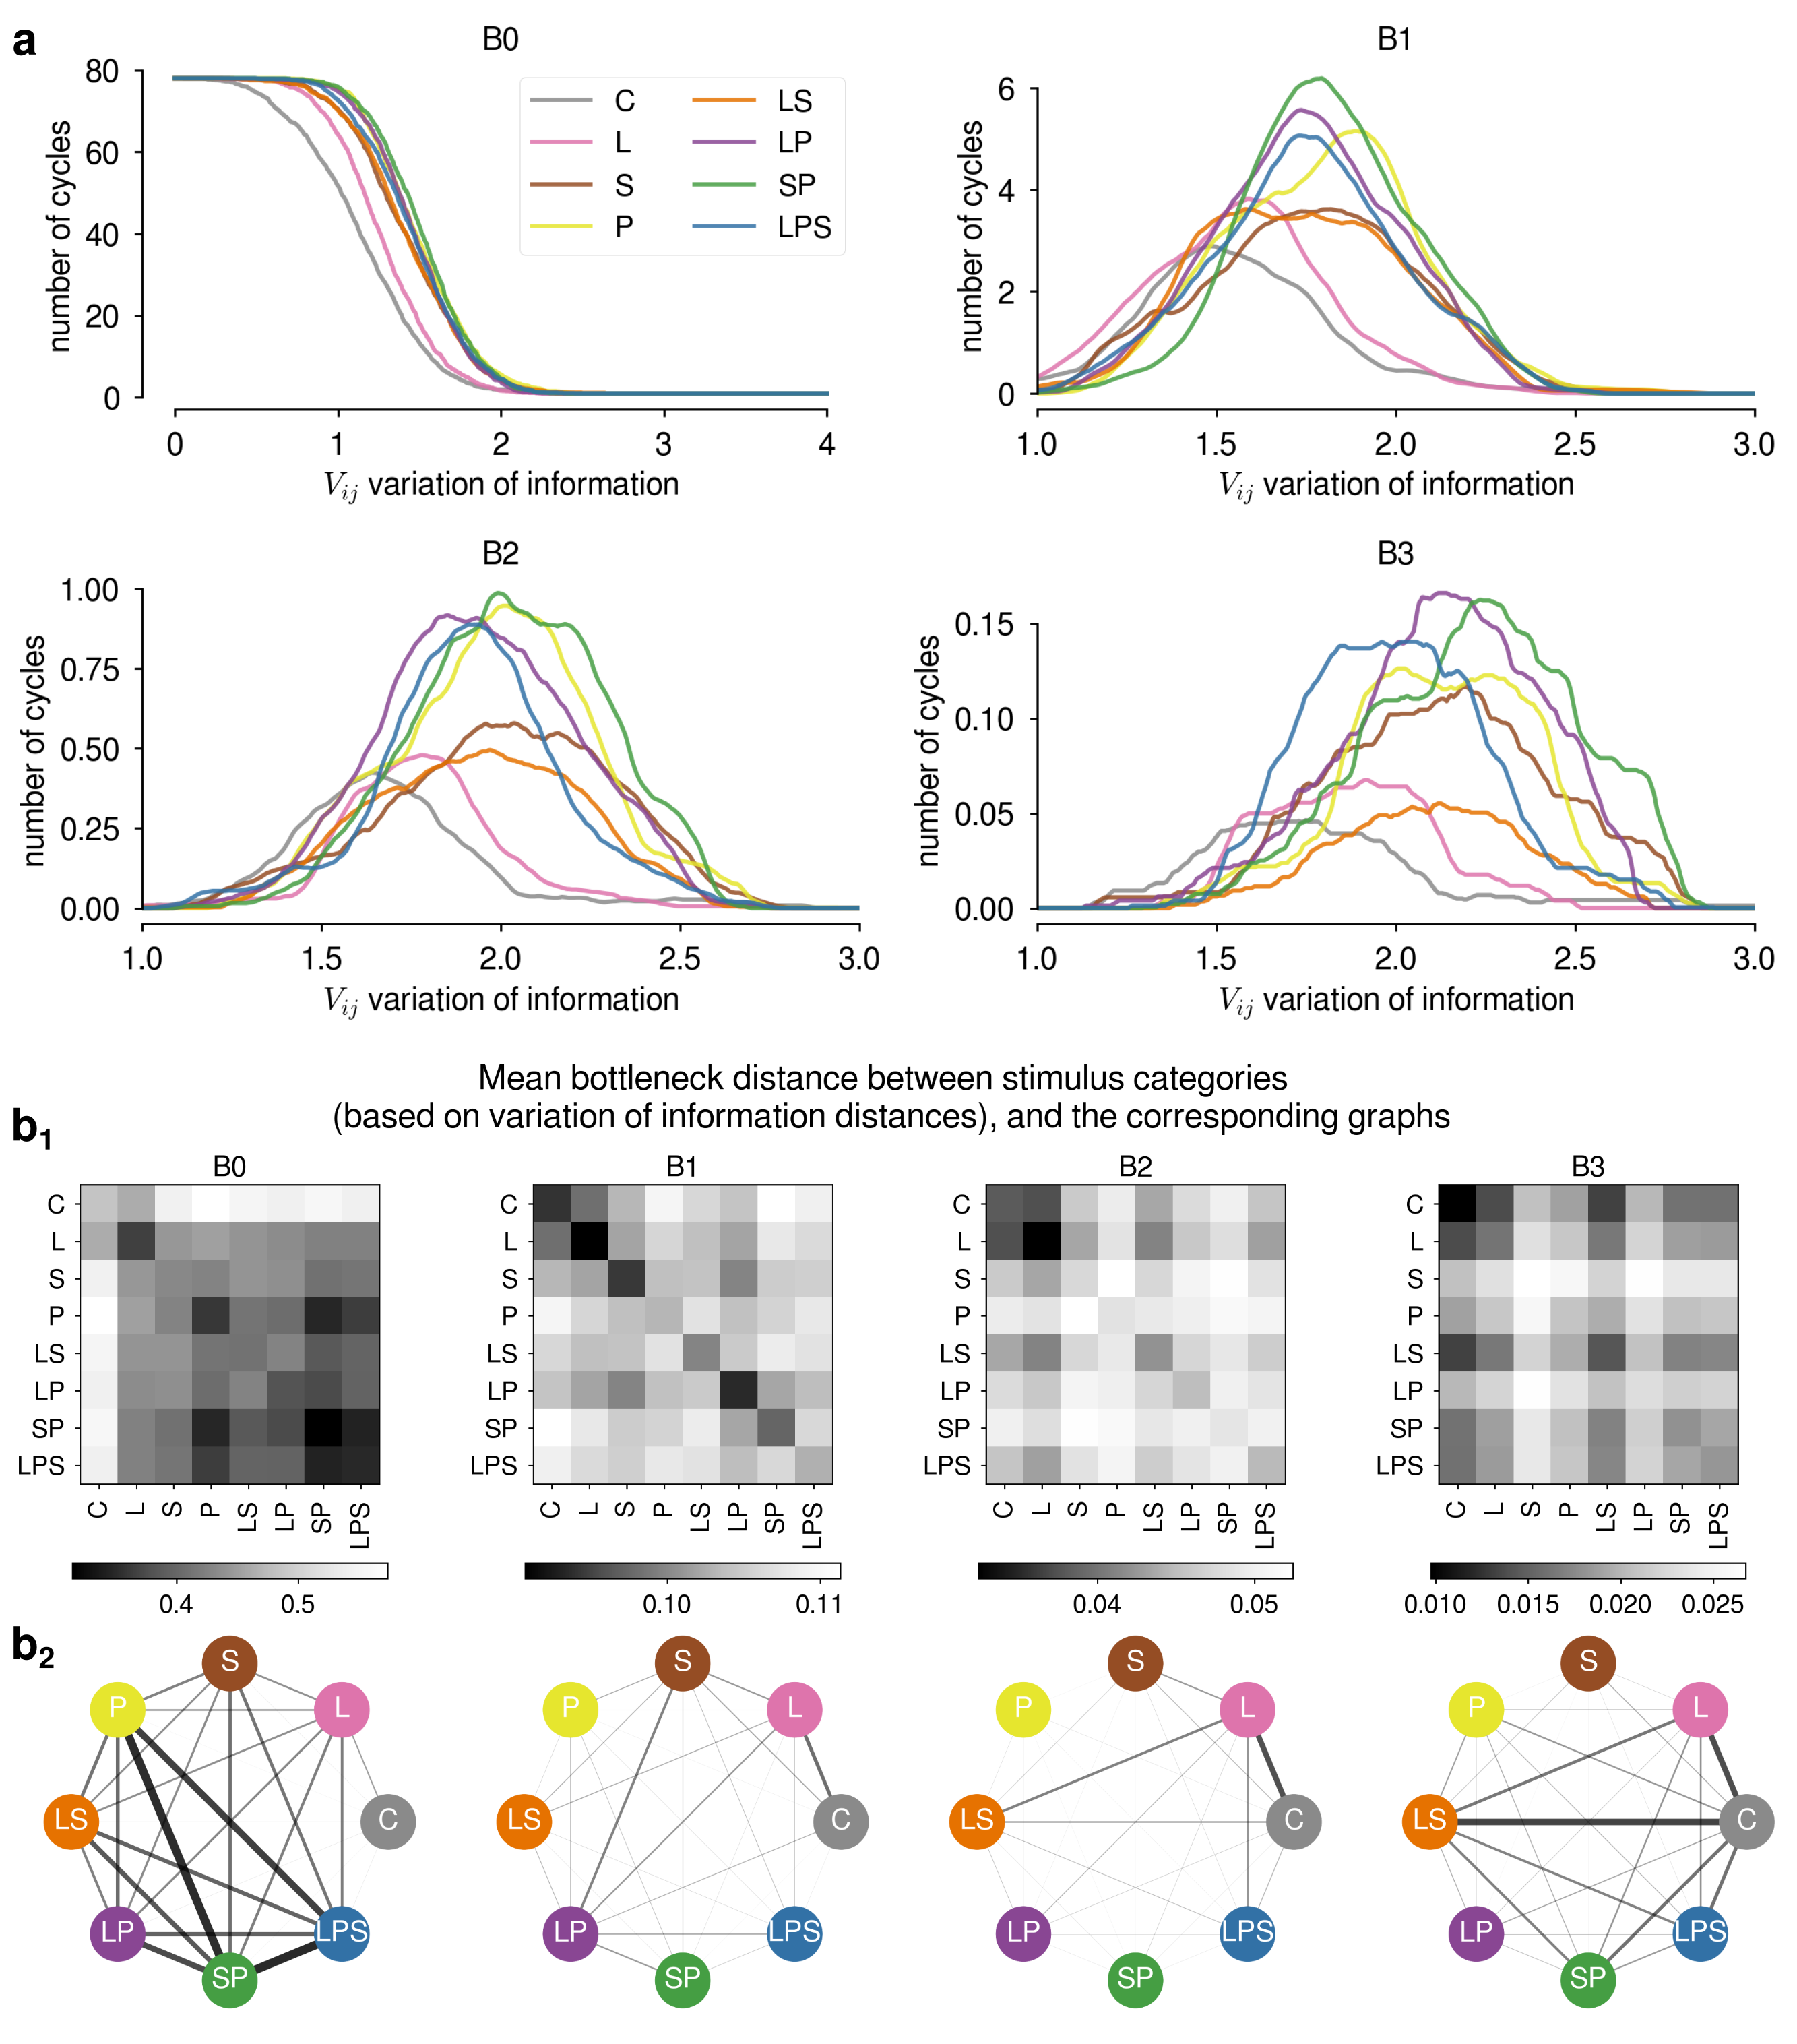
\includegraphics[width=0.6\textwidth,center]{../figures/report/Fig5.png}
    \caption{\label{fig:5}
    \textit{Title}.
    Descriptions
    }
\end{figure}

Roughly similar trends appear under inspection of the persistent scores (\autoref{fig:6}), though it is hard to say with significance due to low number of trials per category. In $B_0, B_1$, integrated Betti number, mean lifetimes and especially persistent entropy generally reveal higher median values than control (C), and sometimes also than light (L). In $B_2$, the effects of P presence is revealed as the four measures are generally higher when the categories contain P (i.e. P, LP, SP, LPS). It is harder to observe trends in $B_3$ for persistent scores. In all of the homology dimensions, the high variability in C might mean there were false positive trials, i.e. some irrelevant responses in the population activity to environment factors or maybe self-movements. This is difficult to assess without behavioral data. Higher number of trials might have blurred that out.

Upon inspection of the bottleneck distances (graphs) between these stimulus categories (\autoref{fig:5}b$_2$), it is clear that C is further from the rest in $B_0,B_1,B_2$ but still closer to L. P is much closer to SP and LPS than the rest especially in $B_0$, but not necessary in other dimensions. In retrospect, a normalization to identity elements in the bottleneck distance matrices might have revealed better structure and relation between these categories. The fact that some of the categories have high self mean bottleneck distances might mean that there is higher variability in the persistent diagrams.

Regardless, these comparisons show that the Betti curves and the persistent features might be useful in recognizing some categories or some modalities, for example at least whether a sensory stimulus is present in a trial versus a control trial. This prompts me to try using these features for classification in the following experiments.

\begin{figure}[H]
    \centering
    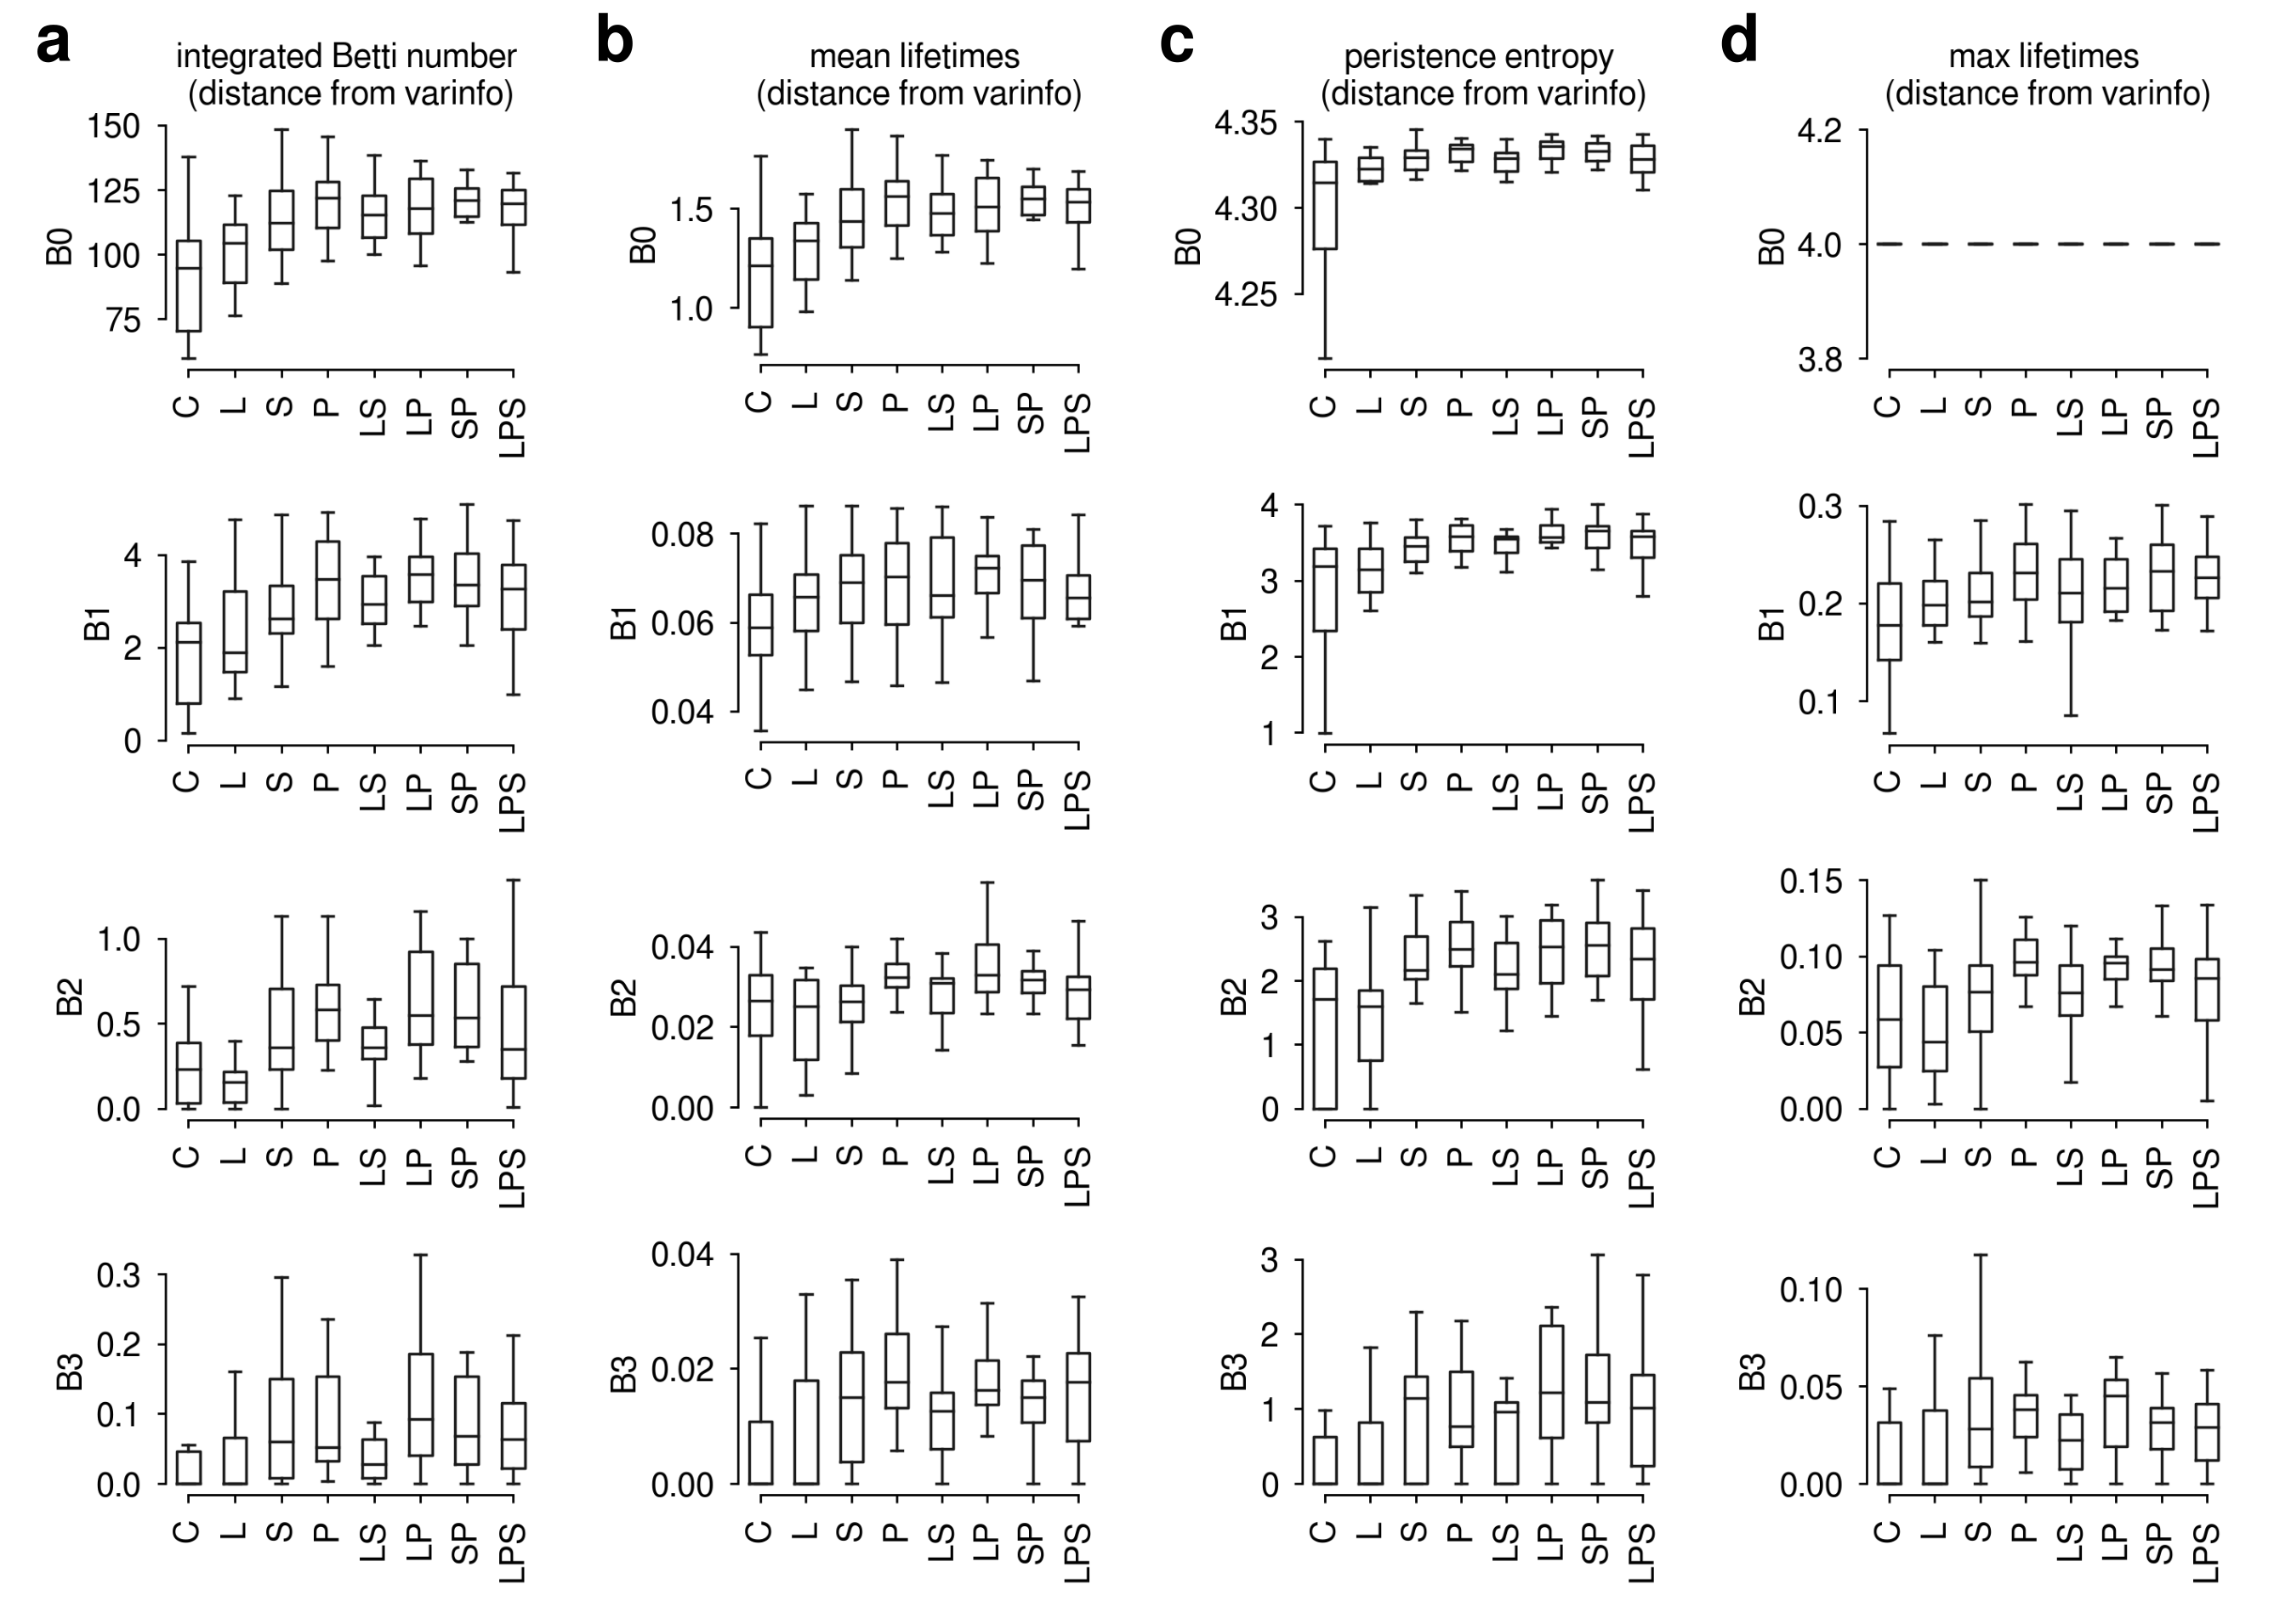
\includegraphics[width=0.75\textwidth,center]{../figures/report/Fig6.png}
    \caption{\label{fig:6}
    \textit{Title}.
    Descriptions
    }
\end{figure}

\subsection{Classification of the different stimulus categories}

For simplicity, I trained a simple MLP network with a single hidden layer with an option for batch-norm layer, trained using two different optimizers (hence 4 different training configurations). The inputs are combinations from the topology analysis and mean activity difference (see Methods). The testing is done in a one-trial-per-category hold-out fashion for 100 times. The reason for including activity features is to establish a baseline performance in which the model can rely on very accessible, easily computable features based directly on the activity.

As a side node, future computational experiments should consider other models (e.g. generalized linear models) and multi-label classification goals (instead of assuming single-label classification).



\begin{table}[h!]
    \centering
\footnotesize
\begin{tabular}{cccccccc}
    \toprule
    \textbf{net-optim} & \multicolumn{7}{c}{\textbf{inputs} constructed on on} \\ \cmidrule{2-8}
    {} & $\Delta$ (avr activ diff) & $\phi$ (pers scores) & $\beta$ (Betti curves) & $\Delta$,$\phi$ & $\Delta$,$\beta$ & $\phi$,$\beta$ &   $\Delta$,$\phi$,$\beta$ \\
    \hline
        mlp-SGD    &           $24.12 \pm 2.60$ &           $17.25 \pm 2.24$ &           $17.38 \pm 2.61$ &  $\mathbf{27.50 \pm 2.84}$ &           $22.12 \pm 2.42$ &  $\mathbf{18.88 \pm 2.36}$ &  $\mathbf{26.50 \pm 2.80}$ \\
        bn-SGD  &           $26.50 \pm 3.27$ &           $17.50 \pm 2.62$ &  $\mathbf{17.75 \pm 2.45}$ &           $26.75 \pm 3.00$ &           $21.50 \pm 2.27$ &           $16.88 \pm 2.33$ &           $21.50 \pm 2.59$ \\
        mlp-Adam   &  $\mathbf{26.75 \pm 2.59}$ &           $18.00 \pm 2.46$ &           $15.12 \pm 2.36$ &           $27.25 \pm 2.93$ &           $21.88 \pm 2.84$ &           $15.12 \pm 2.28$ &           $25.88 \pm 2.38$ \\
        bn-Adam &           $24.00 \pm 2.91$ &  $\mathbf{19.88 \pm 2.57}$ &           $16.25 \pm 2.09$ &           $25.62 \pm 2.89$ &  $\mathbf{22.88 \pm 2.48}$ &           $15.50 \pm 2.19$ &           $23.50 \pm 2.80$ \\
        & & & & & & & [mean $\pm$ CI$_{95}$] \\
    \hline
        mlp-SGD    &           $62.50$ &           $50.00$ &           $50.00$ &           $62.50$ &  $\mathbf{62.50}$ &   $\mathbf{50.00}$ &         $\mathbf{62.50}$ \\
        bn-SGD  &  $\mathbf{75.00}$ &           $50.00$ &  $\mathbf{62.50}$ &  $\mathbf{75.00}$ &           $50.00$ &            $50.00$ &                  $62.50$ \\
        mlp-Adam   &           $62.50$ &           $50.00$ &           $62.50$ &           $62.50$ &           $62.50$ &            $37.50$ &                  $62.50$ \\
        bn-Adam &           $62.50$ &  $\mathbf{75.00}$ &           $50.00$ &           $75.00$ &           $50.00$ &            $50.00$ &                  $50.00$ \\
        & & & & & & & [max] \\
    \bottomrule
\end{tabular}
\normalsize
\caption{\textit{Stimulus classification accuracies after training}
Left columns show the 4 different network configurations (network variants: vanilla vs with batch-norm layer; optimizer variants: SGD vs Adam). The inputs are constructed based on the combinations of 3 different sources: $\Delta$ (mean activity difference before and after stimulus onset), $\phi$ (persistent scores and features) and $\beta$ (concatenated smoothed sub-sampled Betti curves). See Methods for details. The upper table shows the (mean $\pm$ 95\% confidence interval) of 100 instantiations of train-test splitting (one-trial-per-categories held out). The lower table shows the maximum accuracies achieved at the end of the training for each setup. Bold numbers represent the ``best'' in each column per table.
}
\label{table:1}
\end{table}

Results are show in \autoref{table:1}. The ``best'' accuracies across the 4 different training configurations \texttt{net-optim} (i.e. the bold ones per column in the upper table) show that the best mean performance is only a bit better than twice chance (chance is $1/8=12.5\%$). And it is sufficient to use just activity based features $\Delta$ to achieve this. Using persistent scores $\phi$ is moderately better than Betti curves $\beta$ but either way is only better than chance by less than 8\%. The only worthwhile combination comes from activity and persistent scores $(\Delta,\phi)$ by roughly 1\% across the different training configurations, but it might not be significant. Even if a rank significance test is performed, the performance gain is too small. Better feature building based on solely activity might already achieve better increase.

Inspecting the actual maximum achieved accuracies (lower half of \autoref{table:1}) reveals that there are some ``best'' cases where 6 out of 8 categories are correctly classified. And $(\Delta,\phi)$ is not really much better than $\Delta$ alone. Inclusion of Betti curves apparent seems to degrade performance across different training configurations.